\documentclass{article}
\usepackage[utf8]{inputenc}
\usepackage{biblatex}
\usepackage{graphicx}
\usepackage[font=small, labelfont=bf]{caption}
\usepackage{amsmath}
\usepackage{amsthm}
\usepackage{mathabx}
\usepackage{tikz}
\usepackage{esvect}
\usetikzlibrary{automata, positioning, arrows}

\title{Computability: Proof by Construction and Disproof by Contradiction}
\author{Oluwafunke Alliyu, Ethan Balcik, Paul John Balderston, Sen Zhu}
\date{April 2021}

\begin{document}
\theoremstyle{definition}
\newtheorem{exmp}{Example}[section]
\newtheorem{defin}{Definition}[section]

\maketitle

\section{Introduction}
In the age of digital communications, it is difficult to imagine how, in a world without digital computers, one might work toward the development of one.  As a result, often overlooked are the initial developments which led to today's digital age.  Nevertheless, the emergence of digital computers would not be possible without initial, groundbreaking developments in mathematical logic and information theory from significant engineers and mathematicians like Alan Turing and Claude Shannon.  Throughout this paper, we discuss computability in a rigorous, self-contained manner - both its proof by construction and its disproof by contradiction, with examples of each.  Furthermore, we aim to provide our readers with some historical insight into the development of these methods in order to build both an appreciation of their significance, and of the current challenges researchers face as attempts are made to further progress in theoretical computer science \cite{1}.

\section{Background}
Here we introduce the background section
\subsection{Historical Background}
Here we discuss the history behind computer science and its foundations in mathematics
\subsection{Mathematical Logic and Set Theory}
Here we discuss relevant concepts in mathematical logic and set theory
\subsection{Finite State Machines}
Here we discuss finite state machines, state diagrams, etc. to provide the necessary background to understand conceptual machines and understand Turing Machinces graphically

\section{Turing Machines}
An effective model for the general-purpose computer is the Turing Machine, developed by Alan Turing in 1936 \cite{2}.  The Turing Machine is a conceptual model of a general-purpose computing machine which involves the following conceptual components:
\begin{itemize}
	\item A "control box" which stores a finitely-large program
	\item A tape with infinite spaces in which symbols can be stored, read, and written
	\item A read-write mechanism for the tape \cite{3}
\end{itemize}
\begin{figure}[h]
	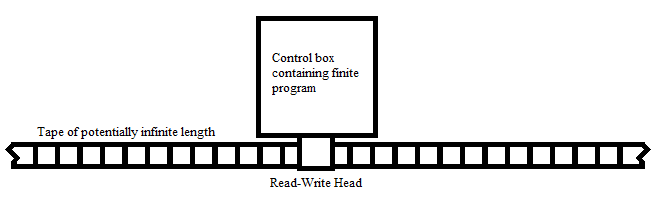
\includegraphics[width=0.85\textwidth]{figure-3-1}
	\centering
	\setlength{\belowcaptionskip}{-10pt}
	\caption{A simple visualization of a Turing machine.  Note that spaces along the tape would be filled with symbols which can be read and written using the read-write head on the machine.}
\end{figure}
\begin{defin}
	A \textbf{Turing Machine} is a 7-Tuple, $(Q, \Sigma, \Gamma, \delta, q_{0}, q_{accept}, q_{reject})$, where:
\end{defin}
\begin{itemize}
	\item $Q$ is a finite set containing the states of the machine
	\item $\Sigma$ is a finite set containing the machine's \textbf{input alphabet}
	\item $\Gamma$ is the finite set containing th emachine's \textbf{tape alphabet} such that the \textbf{blank symbol} $\textvisiblespace \in \Gamma$ and $\Sigma \subseteq \Gamma$
	\item $\delta$ is the \textbf{transition function} $\delta: Q \times \Gamma \to Q \times \Gamma \times \{L, R\}$
	\item $q_{0}$ is the \textbf{starting state} $q_{0} \in Q$
	\item $q_{accept}$ is the \textbf{accept state} $q_{accept} \in Q$
	\item $q_{reject}$ is the \textbf{reject state} $q_{reject} \in Q$ such that $q_{reject} \neq q_{accept}$
\end{itemize}
\noindent A \textbf{configuration} represents the state of a Turing machine's read-write head along its tape, as well as the characters on the tape.  For feasibly-sized tape inputs, a configuration is given as a string of the tape's characters listed starting from the left-most character and working right, with the state $q_{n} \in Q$ inserted to the left of the character currently being read by the read-write head of the machine.  To exemplify this, we can introduce a new instance of a Turing Machine with a specific input, and an algorithm running on the input.
\begin{exmp}
Let's imagine a Turing machine running an algorithm which verifies whether or not a binary string of length $n > 1$ has an even weight (number of 1s in the binary string).  It might achieve this by running the following algorithm:
\begin{enumerate}
	\item Read each bit from left to right on the input string and cross off every other '1' character.
	\item If in step 1 the tape contained no '1' characters, accept.
	\item If in step 1 the tape contained a single '1' character, reject.
	\item Return to the left-most character on the tape.
	\item Return to step 1.
\end{enumerate}
\noindent This particular Turing machine can be given formally as $M = (Q, \Sigma, \Gamma, \delta, q_{1}, q_{accept}, q_{reject})$ such that:
\begin{itemize}
	\item $Q \coloneq \{ q_{1}, q_{2}, q_{3}, q_{4}, q_{5}, q_{accept}, q_{reject} \}$
	\item $\Sigma \coloneq \{ 0, 1 \}$
	\item $\Gamma \coloneq \{ 0, 1, x, \textvisiblespace \}$
	\item The transition function $\delta$ is given as a state diagram (see figure 2)
\end{itemize}
\begin{figure}[h]
	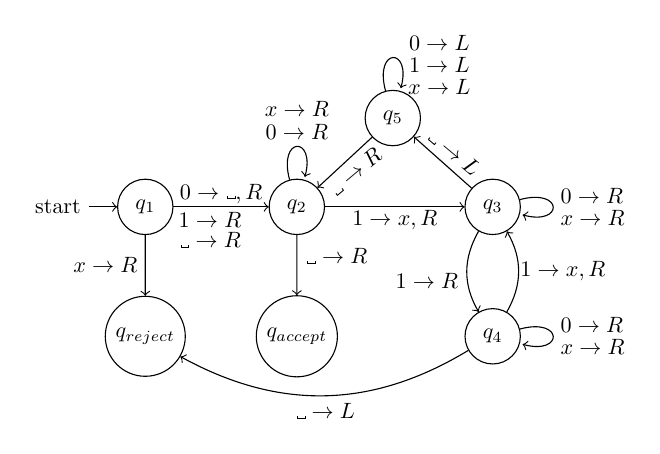
\begin{tikzpicture}[scale=0.8, transform shape]
		\node[state, initial] (q1) {$q_{1}$};
		\node[state, right of=q1, xshift=40] (q2) {$q_{2}$};
		\node[state, right of=q2, xshift=60] (q3) {$q_{3}$};
		\node[state, above left of=q3, xshift=-25, yshift=20] (q5) {$q_{5}$};
		\node[state, below of=q3, yshift=-30] (q4) {$q_{4}$};
		\node[state, below of=q2, yshift=-30] (qaccept) {$q_{accept}$};
		\node[state, below of=q1, yshift=-30] (qreject) {$q_{reject}$};
		\draw[->] (q1) edge node[yshift=6] {\tt $0 \rightarrow \textvisiblespace, R$} node[xshift=-5, yshift=-6] {\tt $1 \rightarrow R$} node[xshift=-5, yshift=-15] {\tt $\textvisiblespace \rightarrow R$} (q2);
		\draw[->] (q1) edge node[xshift=-18] {\tt $x \rightarrow R$} (qreject);
		\draw[->] (q2) edge[loop above] node {\tt $0 \rightarrow R$} node[yshift=10] {\tt $x \rightarrow R$} (q2);
		\draw[->] (q2) edge node[yshift=-6] {\tt $1 \rightarrow x, R$} (q3);
		\draw[->] (q2) edge node[yshift=4, xshift=18] {\tt $\textvisiblespace \rightarrow R$} (qaccept);
		\draw[->] (q3) edge[loop right] node[yshift=-5] {\tt $x \rightarrow R$} node[yshift=5] {\tt $0 \rightarrow R$} (q3);
		\draw[->] (q3) edge[bend right] node[yshift=-4, xshift=-18] {\tt $1 \rightarrow R$} (q4);
		\draw[->] (q3) edge node[rotate=-40, xshift=1, yshift=7] {\tt $\textvisiblespace \rightarrow L$} (q5);
		\draw[->] (q4) edge[bend right] node[xshift=20] {\tt $1 \rightarrow x, R$} (q3);
		\draw[->] (q4) edge[loop right] node[yshift=-5] {\tt $x \rightarrow R$} node[yshift=5] {\tt $0 \rightarrow R$} (q4);
		\draw[->] (q4) edge[bend left,below] node {\tt $\textvisiblespace \rightarrow L$} (qreject);
		\draw[->] (q5) edge node[rotate=40, xshift=1, yshift=-6] {\tt $\textvisiblespace \rightarrow R$} (q2);
		\draw[->] (q5) edge[loop above] node[xshift=21] {\tt $0 \rightarrow L$} node[xshift=21, yshift=-10] {\tt $1 \rightarrow L$} node[xshift=21, yshift=-20] {\tt $x \rightarrow L$} (q5);
	\end{tikzpicture}
	\centering
	\caption{The transition function $\delta$ given as a finite state machine}
\end{figure}
\noindent Using the transition function $\delta$ as given by figure 2, we can show every configuration for a given input string.  For the sake of the example, let's consider the string $\vv{x} = 1101$.  We have the following configurations:
\begin{center}
\begin{tabular}{ c }
	$q_{1}1011$ \\
	$1q_{2}011$ \\
	$10q_{2}11$ \\
	$10xq_{3}1$ \\
	$10x1q_{4}$ \\
	$10xq_{reject}1$
\end{tabular}
\end{center}
\noindent We can clearly see that, since our input string has three '1' characters, our turing machine rejects it.  However, let us walk through each configuration of the input string $\vv{x} = 1001$.  We have the following configurations (read down each column, and then from left to right):
\begin{center}
\begin{tabular}{ c c c c c }
	$q_{1}1001$ & $10q_{5}0x$ & $x0q_{3}0x$ & $q_{5}x00x$ & $x00xq_{2}$ \\
	$1q_{2}001$ & $1q_{5}00x$ & $x00q_{3}x$ & $q_{5} \textvisiblespace x00x$ & $x00x \textvisiblespace q_{accept}$ \\
	$10q_{2}01$ & $q_{5}100x$ & $x00xq_{3}$ & $q_{2}x00x$\\
	$100q_{2}1$ & $q_{5} \textvisiblespace 100x$ & $x00q_{5}x$ & $xq_{2}00x$\\
	$100xq_{3}$ & $q_{2}100x$ & $x0q_{5}0x$ & $x0q_{2}0x$\\
	$100q_{5}x$ & $xq_{3}00x$ & $xq_{5}00x$ & $x00q_{2}x$
\end{tabular}
\end{center}
\end{exmp}
\noindent Now, since our input string has two '1' characters, our turing machine accepts it. \cite{2}

\section{Proof of Computability by Construction}
The outcomes observed in \textbf{Example 3.1} are rather self-evident in the definition of a Turing machine, as two of its parameters are the accept state $q_{accept}$ and the reject state $q_{reject}$.  If a Turing machine ever reaches either of these states, then its algorithm will terminate.  However, a third potential outcome when running an algorithm using a Turing machine is that the algorithm may never terminate.  It is this possibility, the possibility that a Turing machine may run indefinitely for some input, from which much of the theory of computability emerges.  In this section, we will build the definitions which found the theory of computability, and explore how we may prove that a function is computable.
\begin{defin}
	An \textbf{alphabet} is a finite set of arbitrary characters which can be used in some code or language.
\end{defin}
\noindent For example, the english alphabet (ignoring all punctuation and special characters) may define its alphabet as $A_{english} \coloneq \{ a, b, ... , z \}$
\begin{defin}
	A \textbf{word} $\vv{x}$ is a string of characters, each of which belonging to some alphabet $A$.
\end{defin}
\noindent Following from the previous example, we may construct words of varying lengths using the english alphabet, such as "the", "dog", "was", and "running".  Each character composing each of these words belong to the alphabet $A_{english}$ defined above.
\begin{defin}
	A \textbf{language} $L$ is the set of all possible words $\vv{x} \in L$ of varying length, over some alphabet $A$.
\end{defin}
\noindent Any combination of english characters imaginable will certainly be a member of the language $L_{english}$ which is defined on the alphabet $A_{english}$ mentioned previously.
\begin{defin}
	A language $L$ is \textbf{Turing-decidable} if there exists some Turing machine $M$ such that, for each input word $\vv{x} \in L$, $M$ either accepts or rejects it. \cite{2}
\end{defin}
\noindent This definition given is the definition which founds much of the theory of computability.  It does so by use of the Church-Turing thesis, and the wealth of empirical evidence backing it, albeit there is no single, rigorous mathematical proof for this thesis.  Essentially, one interpretation of the thesis states that if one wishes to prove that a certain operation is computable, one can do so by constructing a Turing machine which terminates for all possible inputs into that operation \cite{4}.  (Introduce the operation which we wish to show is computable by construction).

\section{Disproof of Computability by Contradiction}
Definitions/theorems to look into: The Halting Problem, Rice's Theorem; also provide at least one disproof of computability using Rice's Theorem

\section{Conclusions}

\section{References}
\begin{thebibliography}{100}
	\bibitem{1} National Research Council. 1999. Funding a Revolution: Government Support for Computing Research. Washington, DC: The National Academies Press. https://doi.org/10.17226/6323.
	\bibitem{2} Sipser, Michael. 2013. Introduction to the Theory of Computation. Cengage Learning. Third Edition. Print.
	\bibitem{3} Mainzer, Klaus. 2018. Proof of Computation: Digitization in Mathematics, Computer Science, and Philosophy. World Scientific. https://doi.org/10.1142/11005
	\bibitem{4} Evans, David. (2010). Church-Turing Thesis. University of Virginia. Web. http://www.cs.virginia.edu/~evans/cs3102-s10/classes/class15/class15.pdf
\end{thebibliography}

\end{document}